\documentclass{standalone}
\usepackage{tikz}
\usepackage{amsmath}
\usetikzlibrary{positioning}

\tikzset{main node/.style={circle,,draw,minimum size=1cm,inner sep=0pt} }
\begin{document}

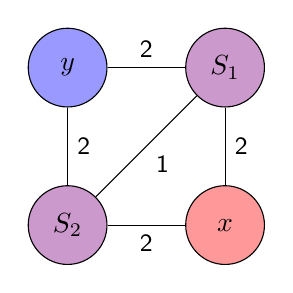
\begin{tikzpicture}
\begin{scope}[on grid]

  \node[main node,fill=blue!40] (1) {$y$};
  \node[main node,fill=violet!40] (2) [right = 2cm of 1] {$S_1$};
  \node[main node,fill=red!40] (3) [below =2cm of 2] {$x$};
    \node[main node,fill=violet!40] (4) [below =2cm of 1] {$S_2$};
 
    \path[every node/.style={font=\sffamily\small}]
    (1) edge [-] node[auto] {2}(2) 
    (1) edge [-] node[auto] {2}(4)
    (2) edge [-] node[auto] {2}(3)
    (2) edge [-] node[auto] {1}(4)
    (3) edge [-] node[auto] {2}(4)
    ;
    \end{scope}
\end{tikzpicture}
\end{document}